\documentclass[12pt]{article}
\usepackage{geometry} %for defining page layout
\geometry{total = {8.5in,11in}, margin=1in}
\usepackage{float}
\usepackage{graphicx}
\graphicspath{ {./images/} }
\usepackage{booktabs} %when copy r code kable()
\usepackage{mathtools} %for aligning proof in classwork

\title{QBS 103: Final Project}
\author{Yihan (Ethan) Zhang}
\date{August 27, 2024}

\begin{document}
\maketitle
\tableofcontents

\newpage
\section{Introduction}
\subsection{Abstract}
The dataset comprises 126 samples, each representing a different individual, and contains expression data for 100 genes. Among these, the gene "ABCA1" was selected for detailed analysis. ABCA1 is a key gene involved in cholesterol metabolism, crucial for generating HDL-C particles that remove cholesterol from cells. Defects in ABCA1, like in Tangier disease, lead to low HDL-C levels and cholesterol buildup, contributing to atherosclerosis. Increasing ABCA1 expression is a potential strategy to reduce the risk of atherosclerotic cardiovascular disease (ASCVD).\cite{Choi2023} The expression values in the dataset are numerical representations of the gene expression levels across different samples, which include various patient characteristics such as age, sex, and ICU status. The primary goal is to visualize the expression patterns of "A1BG" using different types of plots, including bar plots, scatter plots, and box plots, to explore any potential correlations between gene expression and patient characteristics.

\section{Methods}
\subsection{Data Source}
The dataset used for this analysis was obtained from publicly available sources. \cite{Overmyer2021} 
\subsection{R version}
It was processed using R version 3.6.2 (2019-12-12). 
\subsection{R Packages}
Various R packages were employed, including tidyverse for data manipulation and visualization,\cite{Wickham2019} knitr and kableExtra for table formatting,\cite{Zhu2019} pheatmap for generating heatmaps,\cite{Kolde2022} and ggplot2 for creating visualizations.\cite{Tyner2017} 
\subsection{Clustering Algorithm}
The heatmap clustering was performed using the Euclidean distance method, which is well-suited for continuous data such as gene expression levels. Clustering algorithms and color palettes were applied to visualize the patterns and relationships within the data effectively.\cite{Ultsch2022}

\section{Results}
\subsection{Summary Table}
This table provides a summary of demographic and clinical characteristics for patients who were in the ICU compared to those who were not. The variables include age, ferritin levels, CRP levels, sex distribution, and Charlson Comorbidity Scores. The mean age and biomarker levels (ferritin and CRP) are consistent between both groups. However, there are noticeable differences in the distribution of Charlson Scores and sex between the groups, with a higher proportion of males and higher Charlson Scores in the ICU group. (Table \ref{summary table}).

\begin{table}[H]
\centering
\begin{tabular}{lcc}
\toprule
Variable (n(\%)) & In ICU & Not In ICU\\
\midrule
Age & 63.45 (17.82) & 63.45 (17.82)\\
Ferritin (ng/mL) & 935.32 (1067.55) & 935.32 (1067.55)\\
CRP (mg/L) & 149.57 (94.38) & 149.57 (94.38)\\
\addlinespace
\midrule
Sex &  & \\
\midrule
male & 41 (62.12\%) & 33 (55\%)\\
female & 24 (36.36\%) & 27 (45\%)\\
unknown & 1 (1.52\%) & 0 (0\%)\\
\midrule
Charlson Score &  & \\
\midrule
0 & 1 (1.52\%) & 10 (16.67\%)\\
1 & 10 (15.15\%) & 9 (15\%)\\
2 & 14 (21.21\%) & 11 (18.33\%)\\
3 & 13 (19.7\%) & 3 (5\%)\\
4 & 6 (9.09\%) & 9 (15\%)\\
5 & 6 (9.09\%) & 5 (8.33\%)\\
6 & 2 (3.03\%) & 6 (10\%)\\
7 & 8 (12.12\%) & 4 (6.67\%)\\
8 & 3 (4.55\%) & 3 (5\%)\\
9 & 2 (3.03\%) & 0 (0\%)\\
11 & 1 (1.52\%) & 0 (0\%)\\
\bottomrule
\end{tabular}

\caption{Demographic and clinical characteristics of patients stratified by ICU status. This table shows the mean age, ferritin, and CRP levels, as well as the distribution of sex and Charlson Comorbidity Scores among ICU and non-ICU patients.}
\label{summary table}
\end{table}

\subsection{Histogram}
This histogram displays the distribution of expression levels for the gene 'ABCA1' across the dataset. The gene expression levels are varied, with a higher frequency observed at lower expression levels and a tapering frequency at higher expression levels, indicating a right-skewed distribution. (Figure \ref{final_bar_char}).

\begin{figure}[H]
    \centering
    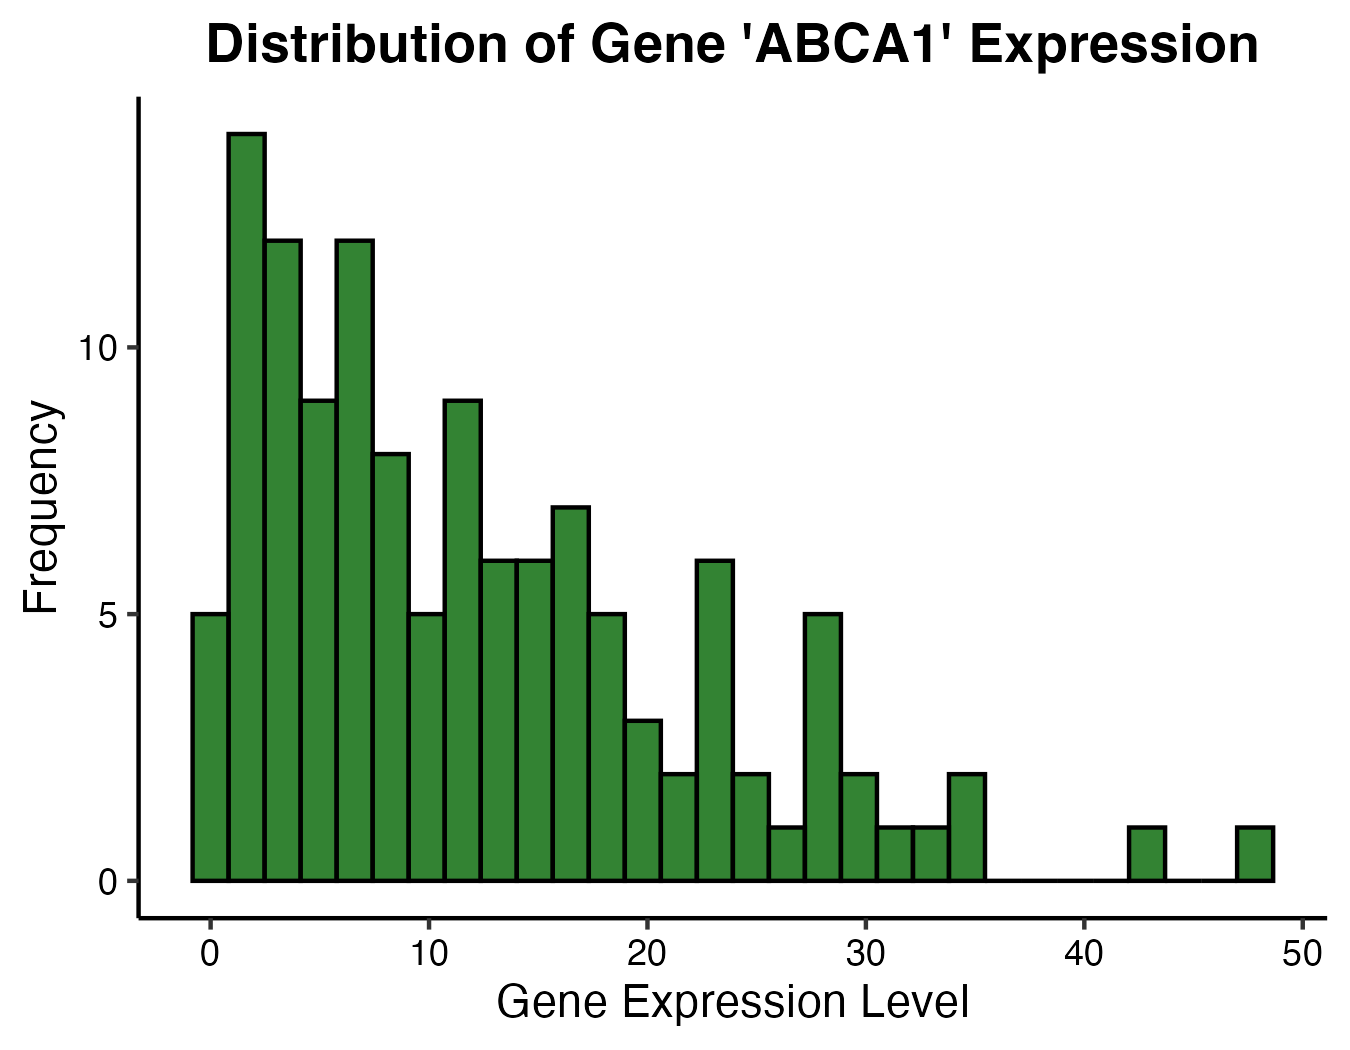
\includegraphics[width=0.7\textwidth, height=0.4\textheight]{final_bar_char.png}
    \caption{Distribution of Gene 'ABCA1' Expression Levels Across the Sample Set.}
    \label{final_bar_char}
\end{figure}

\subsection{Scatter plot}
This scatterplot visualizes the relationship between ABCA1 gene expression levels and participant age. The plot reveals a wide distribution of gene expression levels across different ages, with no clear linear relationship. The color gradient indicates higher gene expression levels in red and lower levels in green, with most data points concentrated in the lower expression range. (Figure \ref{final_scatter}).

\begin{figure}[H]
    \centering
    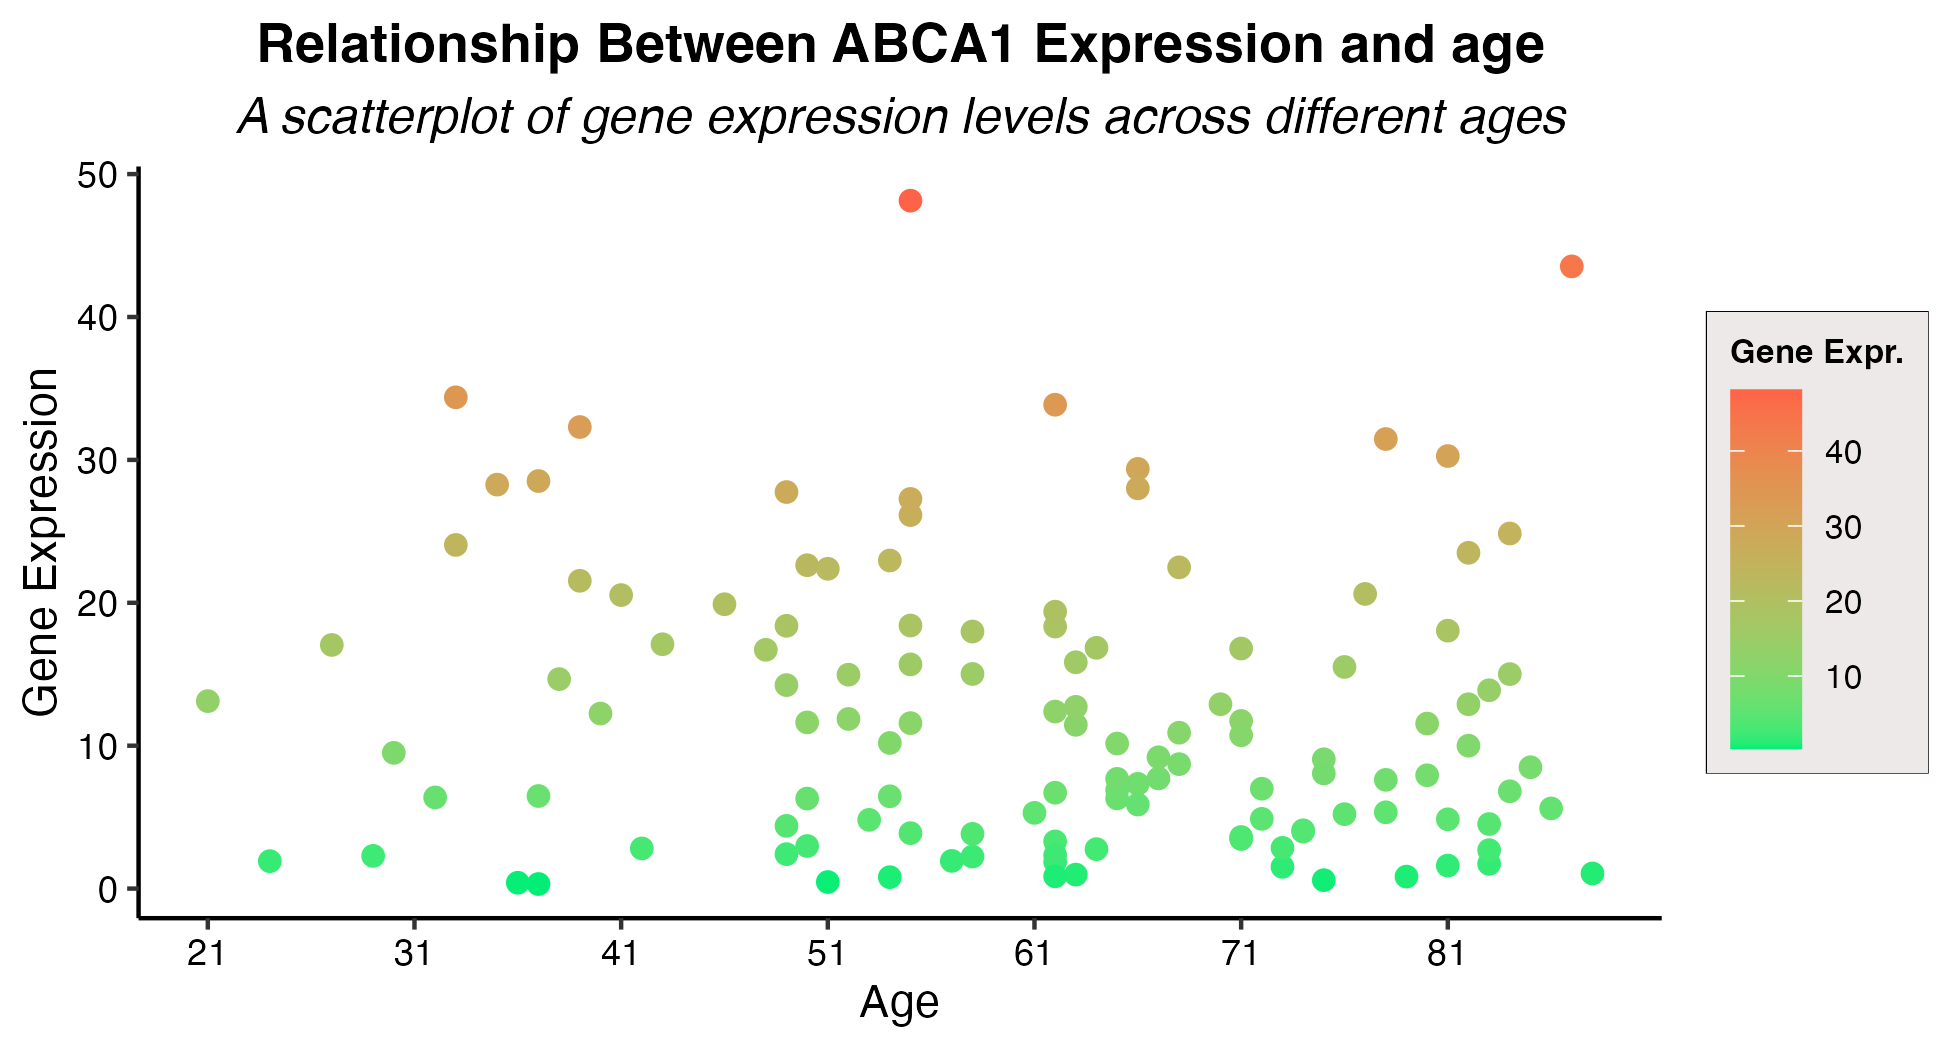
\includegraphics[width=0.7\textwidth, height=0.3\textheight]{final_scatter.png}
    \caption{Scatterplot of ABCA1 Gene Expression Levels Across Different Ages.}
    \label{final_scatter}
\end{figure}

\subsection{Boxplot}
This boxplot compares the distribution of gene expression levels by ICU status and sex. The plot shows that males generally have higher gene expression levels than females, with more variability in the "no ICU" group. The plot also highlights a few outliers, particularly among males in the "yes ICU" group. (Figure \ref{final_box_plot}).

\begin{figure}[H]
    \centering
    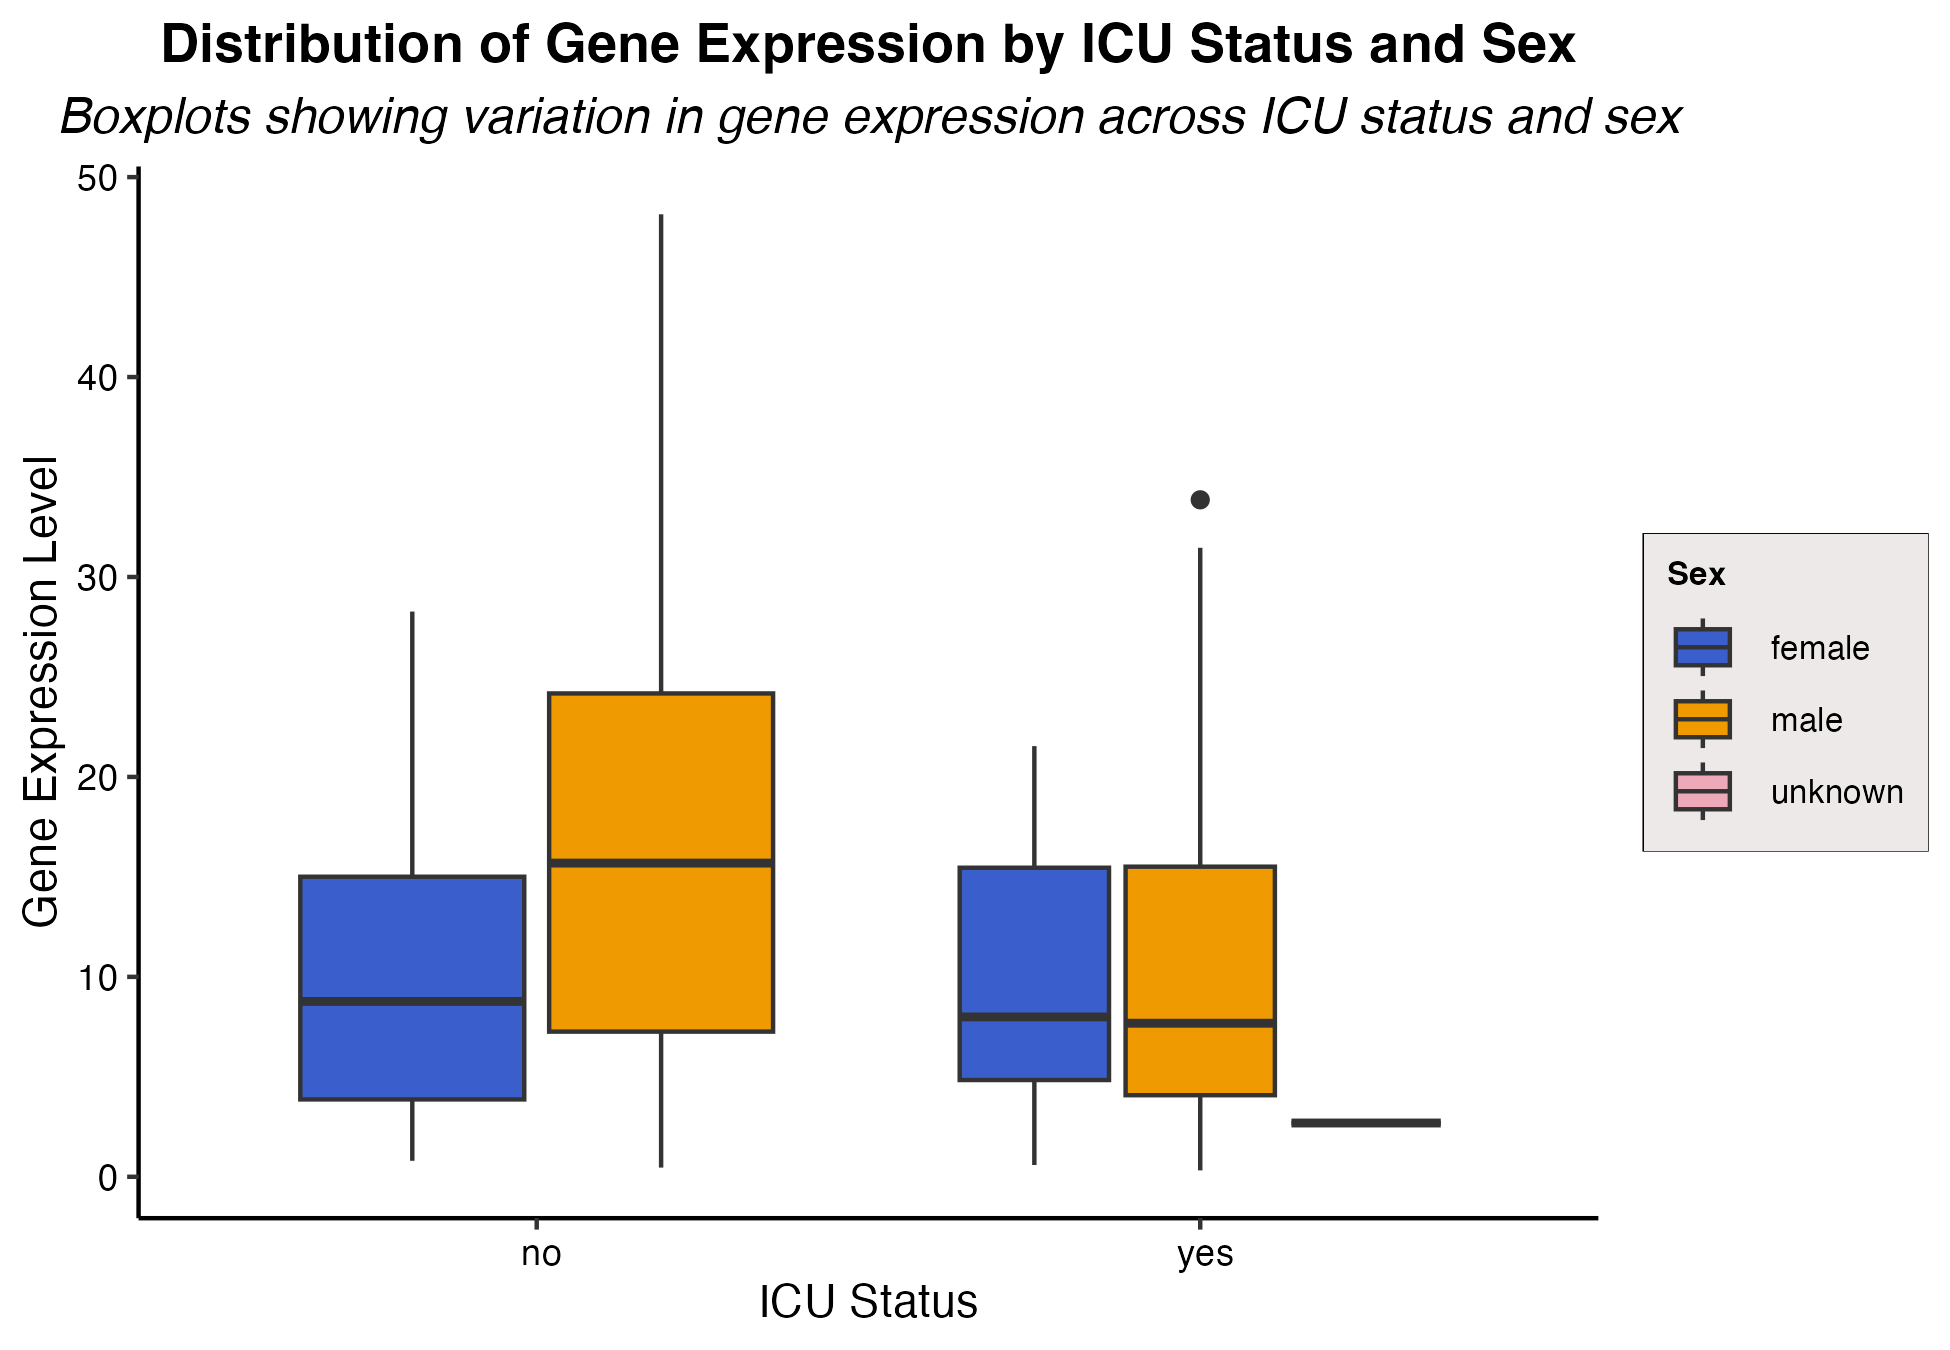
\includegraphics[width = \textwidth]{final_box_plot.png}
    \caption{Boxplot of Gene Expression Levels by ICU Status and Sex, Showing Variation Across Groups.}
    \label{final_box_plot}
\end{figure}

\subsection{Heatmap}
This heatmap visualizes the expression levels of selected genes across different samples, with hierarchical clustering applied to both genes and samples. The color gradient represents gene expression levels, with blue indicating lower expression and red indicating higher expression. The samples are annotated by sex and ICU status, allowing for the identification of patterns or clusters related to these variables. (Figure \ref{final_heatmap}).

\begin{figure}[H]
    \centering
    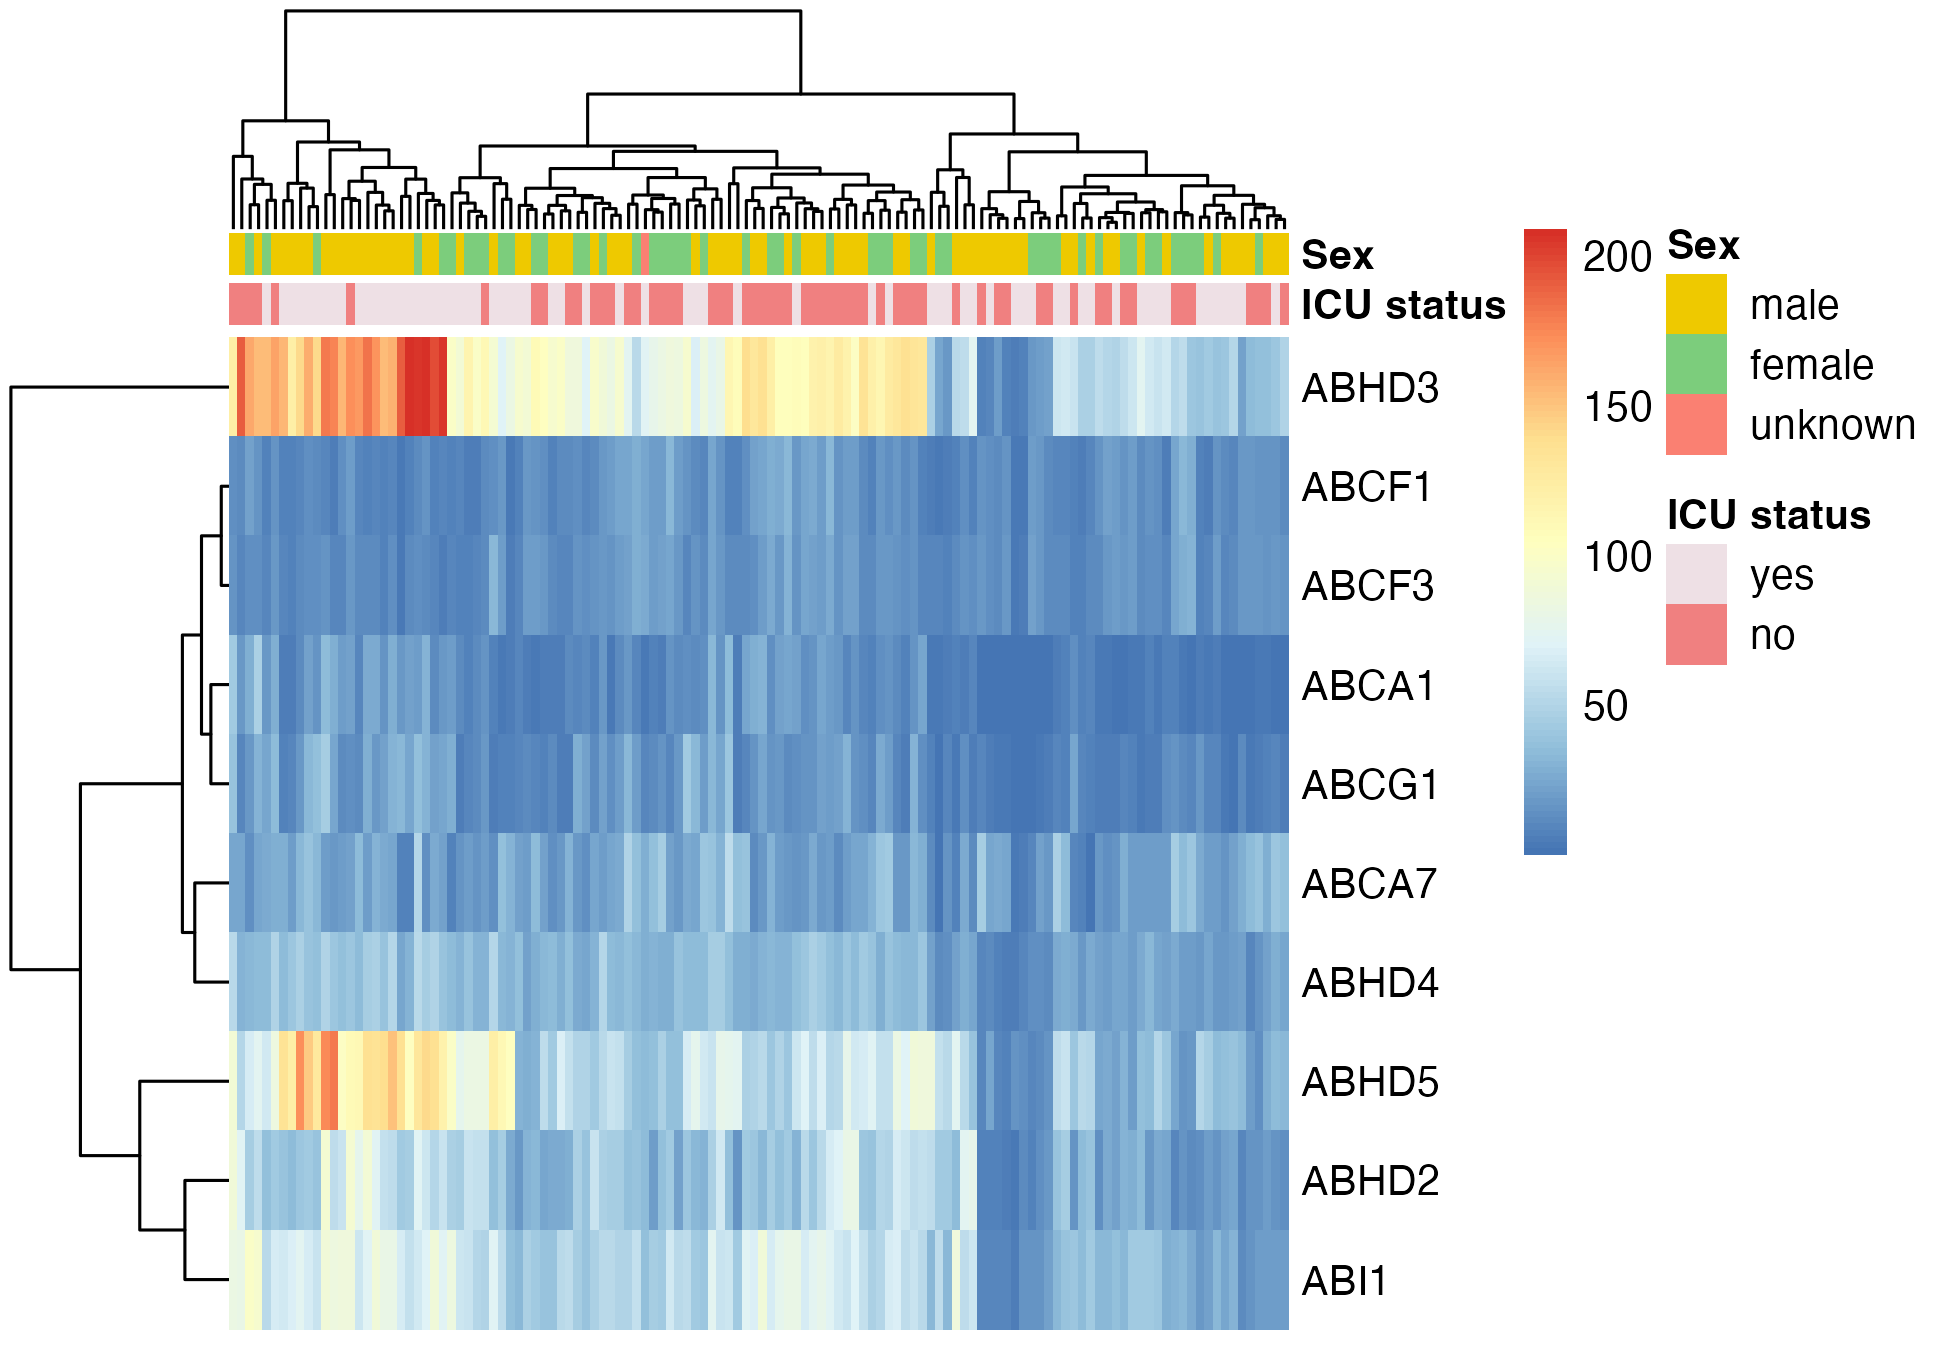
\includegraphics[width=0.9\textwidth, height=0.4\textheight]{final_heatmap.png}
    \caption{Heatmap of Gene Expression Levels with Hierarchical Clustering by Sample and Gene, Annotated by Sex and ICU Status.}
    \label{final_heatmap}
\end{figure}

\subsection{Violin Plot}
The violin plot displays the distribution of gene expression levels for males and females. The plot reveals that males tend to have a wider range and higher levels of gene expression compared to females. (Figure \ref{final_violin_plot}).

\begin{figure}[H]
    \centering
    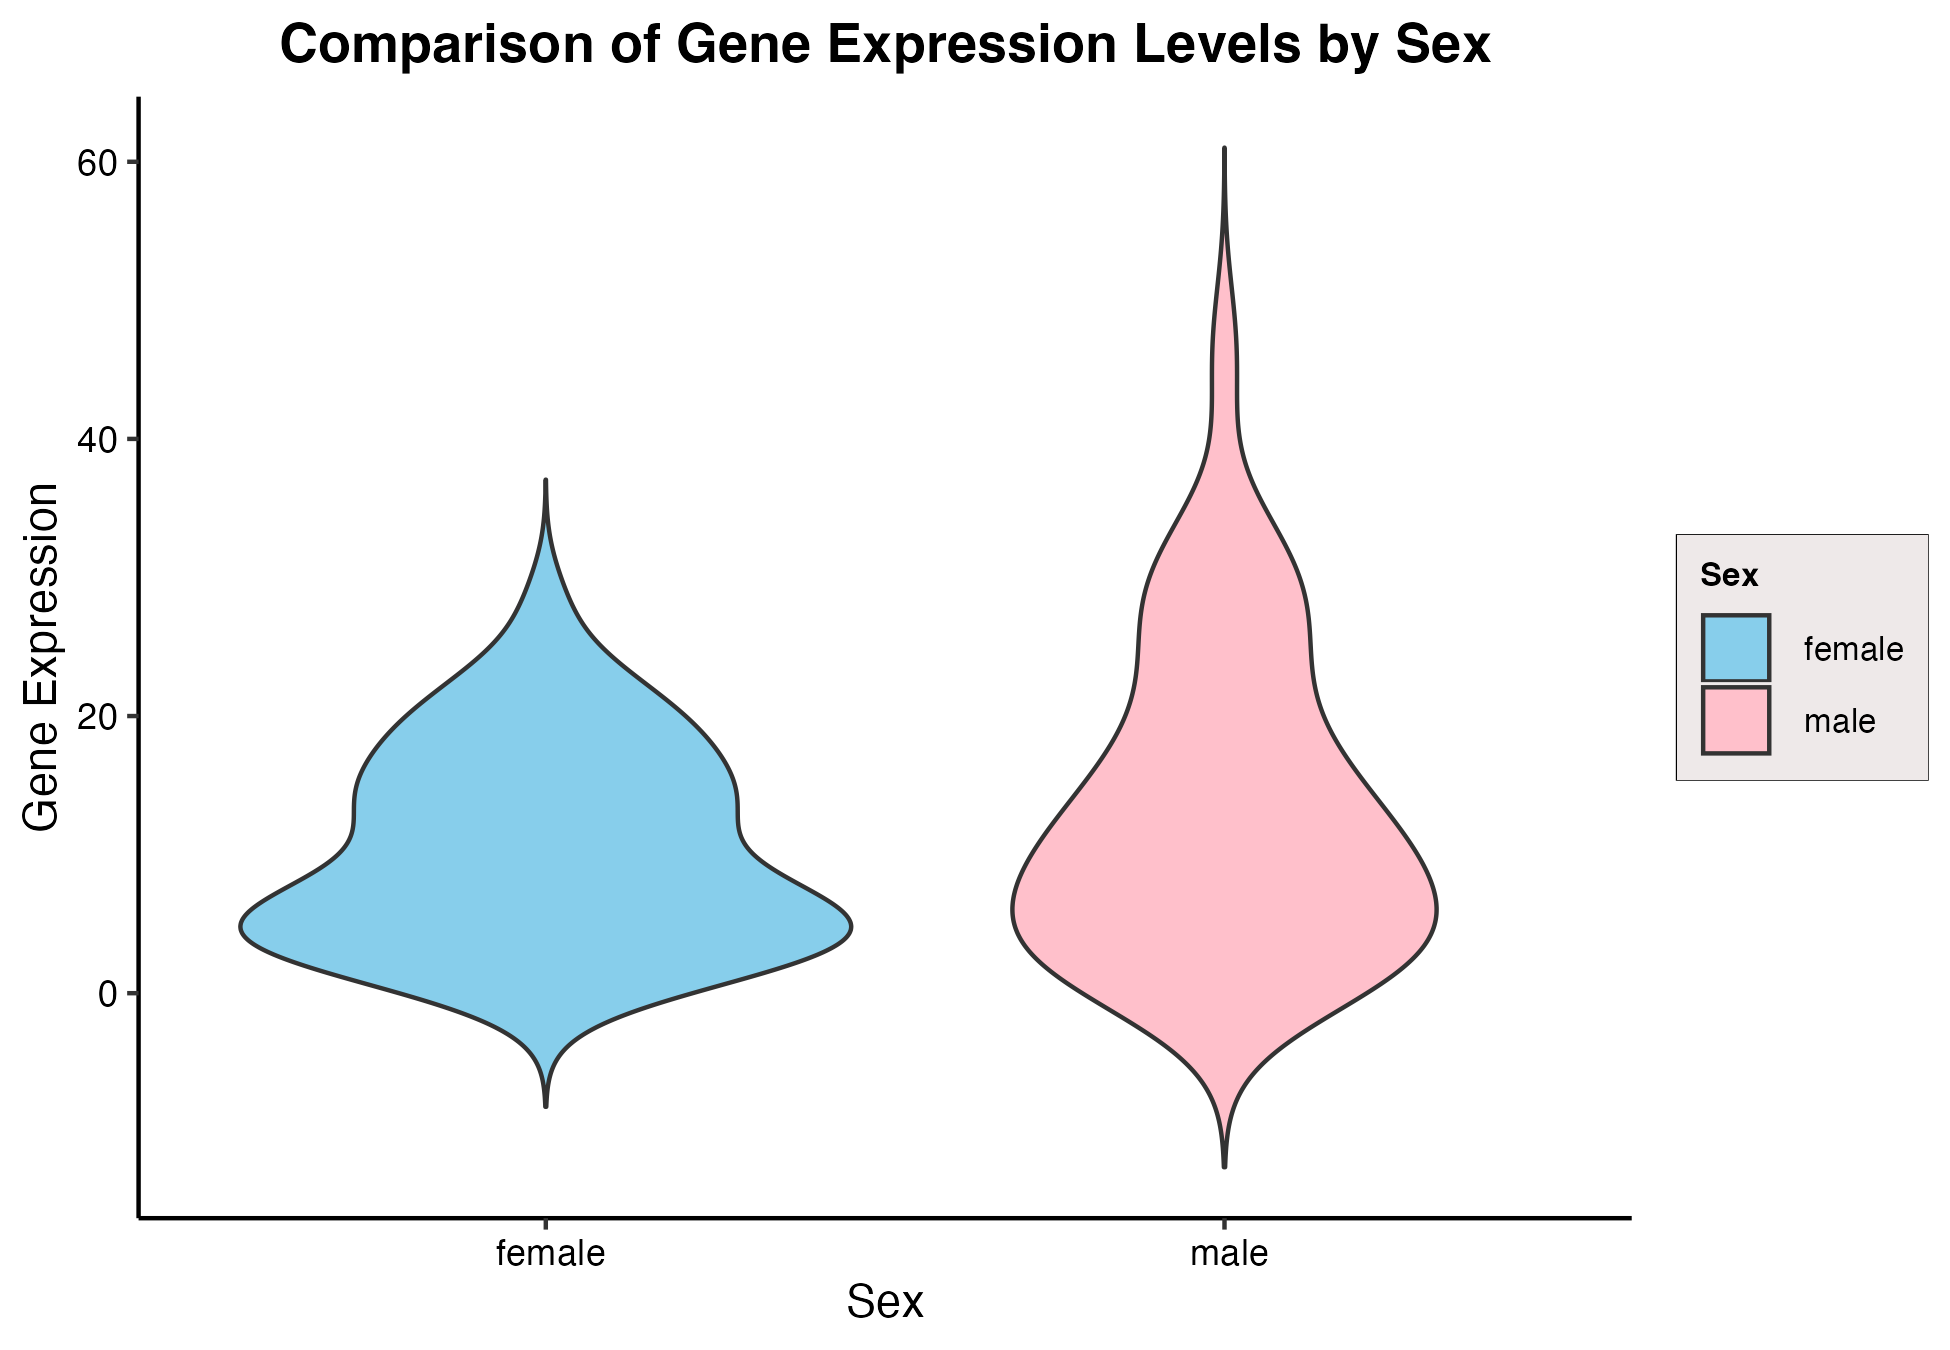
\includegraphics[width=0.6\textwidth, height=0.3\textheight]{final_violin_plot.png}
    \caption{The plot shows that males generally exhibit a broader range and higher gene expression levels compared to females.}
    \label{final_violin_plot}
\end{figure}

\newpage
\bibliographystyle{pnas2009}
\bibliography{export_zyh}

\end{document}
